\documentclass[omni.tex]{subfiles}

\begin{document}

\begin{figure}
{\begin{center}
    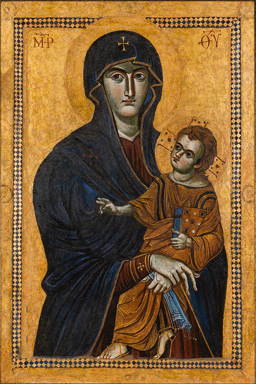
\includegraphics[width=2in]{salus_populi_romani}
\end{center}}
\end{figure}

\poemtitle{Ave Mar\'ia}
\settowidth{\versewidth}{Et ne nos ind\'ucas in tentati\'onem}

\begin{verse}[\versewidth]
\lettrine[lhang=1.0,nindent=0em]{A}{ve Mar\'ia}, \\>
gr\'atia plena,\\>
D\'ominus tecum: \\
bened\'icta tu in muli\'eribus, \\
et bened\'ictus fructus ventris tui, \\
Iesus.
\end{verse}

\begin{verse}[\versewidth]
Sancta Mar\'ia, \\
Mater Dei, \\
ora pro nobis peccat\'oribus, \\
nunc et in hora mortis nostr\ae. \\
Amen. \\[4\baselineskip]
\end{verse}
\attrib{II}

\pagebreak
\end{document}
